\section{Introduction}

\subsection{Contexte}
\begin{frame}{Contexte}
Ces dernières années plusieurs catastrophes sont dues à des erreurs de spécifications des systèmes développés.
\begin{columns}
	\begin{column}{0.3\textwidth}
		\begin{figure}
			\begin{tikzpicture}		
			\only<2->
			{
				\node [inner sep=-10pt]
				{
					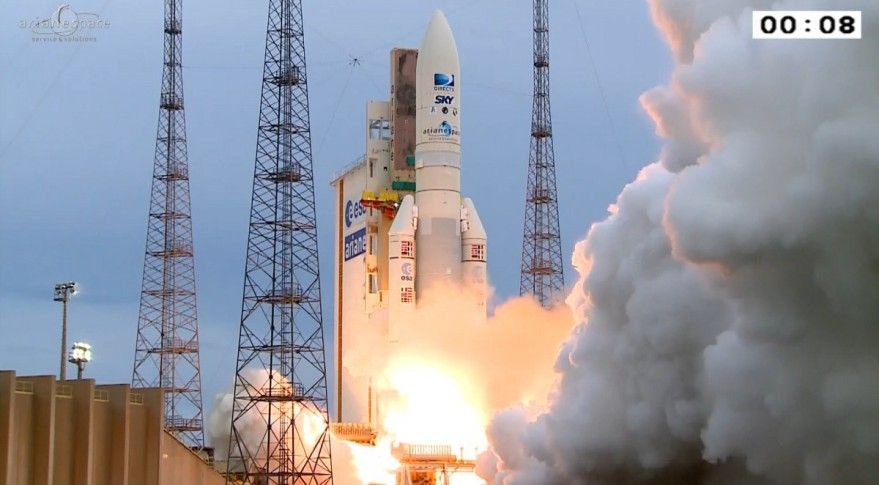
\includegraphics[height=1.2in,width=\columnwidth,trim={0 0 0 0},clip]{resources/Ariane_5}
				};              
			}
			\end{tikzpicture}
			\onslide<2->
			{  
				\caption{Ariane 5}
			}
		\end{figure}
	\end{column}

	\begin{column}{0.3\textwidth}
	\begin{figure}
		\begin{tikzpicture}		
		\only<3->
		{
			\node [inner sep=-10pt]
			{
				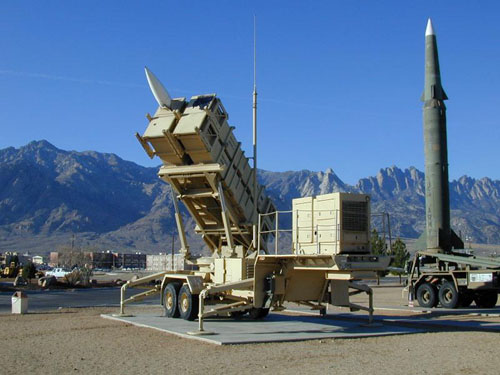
\includegraphics[height=1.2in,width=\columnwidth,trim={0 0 0 0},clip]{resources/Patriot}
			};              
		}
		\end{tikzpicture}
		\onslide<3->
		{  
			\caption{Missile Patriote}
		}
	\end{figure}
\end{column}

	\begin{column}{0.3\textwidth}
		\begin{figure}
			\begin{tikzpicture}
			\only<4->
			{
				\node [inner sep=-10pt]
				{
					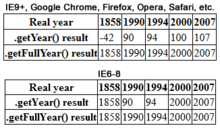
\includegraphics[height=1.2in,width=\columnwidth,trim={0 0 0 0},clip]{resources/bug2000}
				};
			}
			\end{tikzpicture} 
			\onslide<4->
			{
				\caption{Bug 2000}
			}
		\end{figure}
	\end{column}            
\end{columns}

\uncover<5->{%
La fiabilité de tout système est envisageable, en particulier ceux de systèmes critiques.
}
%Vue l'importance de ces systèmes a complexité de ces systèmes il est pratiquement impossible de s'assurer que le système est fiable. 
\end{frame}

%La necessite d'utiliser les methodes formelle 
\begin{frame}{titre section}
\centering
\vspace{2.2cm}       
	\Huge 
		\textbf{Comment faire?}
%sachant que les jeux de test ne permet pas d'aboutir à une preuve contrainte
\end{frame}

\begin{frame}{titre section}
le model checking permet de détecter automatiquement des erreurs dans le processus de
conception, elle fournit aussi un contre-exemple en cas de non insatiabilité de la propriété dans le modèle permettant ainsi de corriger la source de l’erreur dans le
système.

  \begin{tikzpicture}
  \matrix (magic) [matrix of nodes,ampersand replacement=\&, column sep=7mm, row sep=5mm]{
  	\node (s) [draw,shape=rectangle,visible on=<2->] {Systèmes}; \&
  	\node (sf) [draw,shape=rectangle,visible on=<3->] {Specification du système}; \&
  	\node (ge) [draw,shape=circle,size=20pt,visible on=<4->] {Generations de l'espace d'etats}; \\
  };
  \draw[->, thick,visible on=<3->] (s) -- (sf); 
  \draw[->, thick,visible on=<4->] (sf) -- (ge); 
  \end{tikzpicture}
\end{frame}


\subsection{Motivation}
\begin{frame}{Motivation}
\begin{block}{formales System}
	Ein System welches Regeln enthält, mit deren Hilfe sich mathematische Aussagen beweisen lassen und mit denen aus bereits bewiesenen Aussagen neue Aussagen abgeleitet werden können.
\end{block}
\begin{block}{widerspruchsfrei}
	\begin{itemize}
		\item $A$ Aussage
		\item $T$ formales System
	\end{itemize}
	$$\neg\exists A: T\rightarrow{}A \wedge T\rightarrow{}\neg{}A $$
\end{block}
\end{frame}

\subsection{Objectifs}
\begin{frame}{Objectifs}
\begin{block}{formales System}
	Ein System welches Regeln enthält, mit deren Hilfe sich mathematische Aussagen beweisen lassen und mit denen aus bereits bewiesenen Aussagen neue Aussagen abgeleitet werden können.
\end{block}
\begin{block}{widerspruchsfrei}
	\begin{itemize}
		\item $A$ Aussage
		\item $T$ formales System
	\end{itemize}
	$$\neg\exists A: T\rightarrow{}A \wedge T\rightarrow{}\neg{}A $$
\end{block}
\end{frame}